
\documentclass[onehalf,11pt]{beavtex}
\title{The Meaning of Life}
\author{John Smith}
\degree{Doctor of Philosophy}
\doctype{Dissertation}
\department{Electrical Engineering and Computer Science}
\depttype{School}
\depthead{Director}
\major{Computer Science}
\advisor{Joan Smythe}
\submitdate{September 23, 2011}
\commencementyear{2012}
\abstract{This is an abstract statement.}
\acknowledgements{I would like to acknowledge the Starting State and the Transition Function.}

\usepackage{algorithm}
\usepackage{algorithmic}
\usepackage{graphicx}
\usepackage{grffile}
\usepackage{amsmath}
\usepackage{amssymb}
\usepackage{times}
\usepackage{epsfig}
\usepackage{breqn}
\usepackage{url}
\usepackage[lined,boxed,commentsnumbered,algo2e]{algorithm2e}



\begin{document}
\maketitle

\mainmatter

\chapter{Introduction}
\section{Introduction to the Variant Annotation}

\section{Definition}
\subsection{Gene Structure}

\subsection{Potential Variant Effects}
\begin{figure}[!ht]
\centering
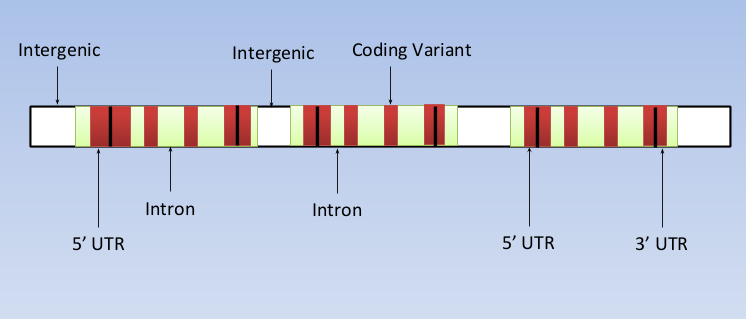
\includegraphics[scale=0.6]{./pic/type.png}
\caption{potential variant functional regions}
\label{fig:variant_effect} 
\end{figure}

In this project, we annotate 7 potential variant effects. The corresponding functional regions are show in Figure \ref{fig:variant_effect}
\begin{itemize}
  \item Intergenic variant \\
  Intergenic variant does not reside in any genes, resulting in that it does not alter any amino acid sequences. So its putative impact is low. 
  \item Intron variant \\
  Intron variant resides in a gene, but not in an exon. Thus, it does not alter any amino acid either. Its putative impact is still low but a little higher than Intergenic variant.
  \item 5' UTR variant \\
  5' UTR variant resides in an exon, but is prior to the start of coding sequence. Although it still does not alter any amino acid sequences, it is relatively more damaging than intergenic and intron variant.
  \item 3' UTR variant \\
  3' UTR variant resides in an exon, but after the stop codon of coding sequences. The putative impact is similar to 5' UTR variant.
  \item Non-coding exon variant \\
  Non-coding exon variant resides in an exon. But the corresponding gene has no start or stop codon, resulting in no coding sequences. Thus, no amino acid sequences would be altered.
  \item Synonymous variant \\
  Synonymous variant resides in an exon and coding sequences, leading to altering a coding sequence. However, since several DNA codons correspond to one amino acid, the resulting amino acid sequence does not change.
  \item Non-synonymous variant \\
  Non-synonymous variant resides in coding sequences and alters an amino acid sequence. Its putative impact is high.
\end{itemize}

The following table shows the notation and putative impact for each variant effect.


\begin{table}[H]
%\label{tab:features}
\centering
\begin{tabular}{l| l}
\hline
Variant effect & Putative impact \\
\hline
  intergenic\_region & MODIFIER \\
  intron\_variant & MODIFIER \\
  5\_prime\_UTR\_variant & MODIFIER \\
  3\_prime\_UTR\_variant & MODIFIER \\
  non\_coding\_exon\_variant & MODIFIER \\
  synonymous\_variant & LOW \\
  non\_synonymous\_variant & MODERATE \\

\end{tabular}
\end{table}

For non-synonymous variant, we annotate the reference amino acid, alternate amino acid and the position of the amino acid instead of the term.


\chapter{Methods}

\section{Input}

\subsection{Genome data}
The genome data contains the whole nucleotide sequences of each chromosome. It is often stored in a faidx-indexed reference file in the FASTA format. We will use this file to get the amino acid codon of a given variant.
Example:

\begin{figure}[!ht]
\centering
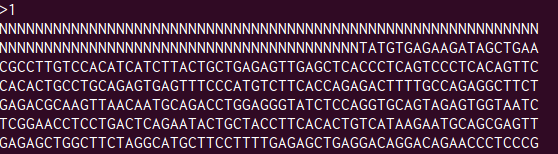
\includegraphics[scale=0.8]{./pic/genome.png}
\caption{Genome data example}
\end{figure}

\subsection{Gene structure data}
The gene structure data contains information about gene structure, such as start codon, stop codon, exon, strand and gene id. This is the key data to determine the functional region of a given variant. Example:

\begin{figure}[!ht]
\centering
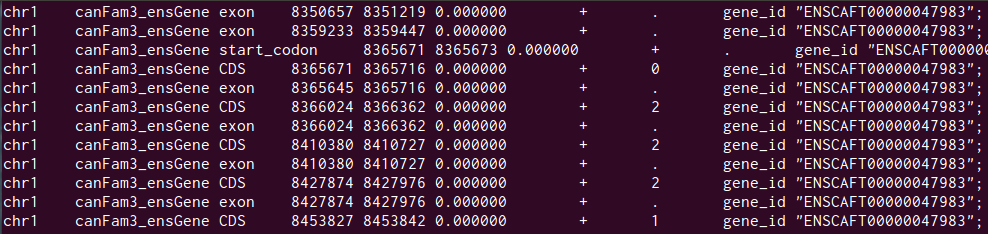
\includegraphics[scale=0.6]{./pic/gtf.png}
\caption{GTF file example}
\end{figure}




\subsection{Variant data}
This is the data to be annotated. The key information includes chromosome, position, reference base and alternate variant alleles of the variant. The data is typically stored in VCF file. We will annotate the variant in the INFO field. Example:
\begin{figure}[!ht]
\centering
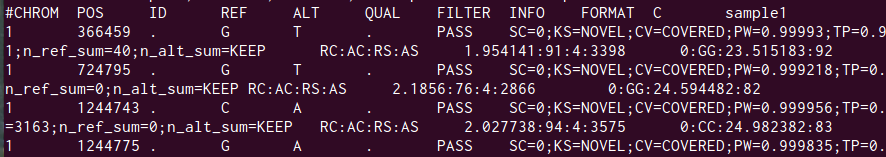
\includegraphics[scale=0.6]{./pic/vcf.png}
\caption{VCF file example}
\end{figure}


\section{Output}
Genes may overlap. Hence, one variant may have several effects. For each variant, the output is a list of effects. The potential effects are listed in section 1.1. In the project, the output is stored in a VCF file in the INFO field. To be specific, a new subfield, named ANN, will be appended to INFO field. The most important information is the effect of variants and the putative impact of the effect.

Besides the effect of variants, the corresponding Ensemble transcript id and common gene name are also annotated. All the annotation formats follow the standard variant annotation in VCF format. Example:
\begin{figure}[!ht]
\centering
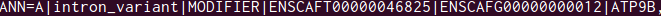
\includegraphics[scale=0.7]{./pic/ann.png}
\caption{VCF file example}
\end{figure}

\section{How it works}
There are 3 datasets to be kept track of. If we search on the whole datasets for each variants, the total running time complexity is O(m*n*k), where m, n and k is the size of each file. In addition, the size of the datasets may be too large to load them all into RAM. For instance, the size of a typical human genome file is about 3.0 GB. To solve the difficulties in this problem, we develop several algorithms to annotate variants.

The whole problem can be split into 2 smaller subproblems. The first one is to obtain a list of genes in which a variant resides. The second one is to annotate each functional region. And if the variant resides in a coding sequence, get the corresponding DNA sequence around the variant and translate it into amino acids.

The most challenging part is to get the gene list since genes may overlap. The naive solution is to search on the whole genome for each gene, resulting in a time complexity of $O(N*K)$, where $N$ is the number of genes and $K$ is the number of variants. To speed up the annotation, 2 algorithms were proposed. One algorithm is array based and efficient for sorted variants while the other is tree based and efficient for unsorted variants.

\subsection{Outline of the algorithm}
\IncMargin{1em}
\begin{algorithm}[h!]
 \label{alg:alg_outline}
 \SetAlgoLined
 \SetKwData{Left}{left}\SetKwData{This}{this}\SetKwData{Up}{up}
 \SetKwInOut{Input}{input}\SetKwInOut{Output}{output}
 \Input{gene structure data $G$. reference genome data $R$. variant data $V$.}
 \Output{The annotated variant data $V$}

     \BlankLine
     \For {each variant v in V at chromosome chr and position pos}{

	  	$gene\_list$ = get\_gene\_list($G$, $chr$, $pos$)
	  	\BlankLine
	  	$A$ = $\varnothing$
	  	
	  	\If{ gene\_list is empty }{
	  		$A$ = $A$ + "intergenic\_region"
	  	}
	  	\BlankLine
	  	
	  	\For { each gene in gene\_list } {
	  		\If{ gene has neither start codon nor stop codon}{
	  			$A$ = $A$ + "non\_coding\_exon\_variant"
	  		}
	  		\ElseIf{v does not reside in any exon of gene}{
	  			$A$ = $A$ + "intron\_variant"
	  		}
	  		\ElseIf{v resides prior to start codon of gene}{
	  			$A$ = $A$ + "5_prime\_UTR\_variant"
	  		}
	  		\ElseIf{v resides after stop codon of gene}{
	  			$A$ = $A$ + "3_prime\_UTR\_variant"
	  		}
	  		\Else{
	  			get reference amino acid $ra$ and alternative amino acid $aa$\\
	  			\If{ $ra$ == $aa$ }{
	  				$A$ = $A$ + "synonymous\_variant"
	  			}
	  			\Else{
	  				$A$ = $A$ + "$ra$ + $pos$ + $aa$"
	  			}
	  		}
	  	}
	  	\BlankLine
	  	Annotate $v$ with $A$
     }
     \BlankLine
     \textbf{return} The annotated variants $V$
 \caption{\textsc{Variant Annotation}}
\end{algorithm}\DecMargin{1em} 

\subsection{Searching algorithm}
2 algorithms are proposed for searching gene list. One is array based and most efficient for sorted variants while the other is tree based and most efficient for unsorted variants.
\subsection{Array based searching}
Array based search algorithm is most efficient for sorted variants. Genes are stored in sorted order in an array. While iterate though the variants, the algorithm keep track of the last visited gene. Each variant start searching from the last visited gene, not from the beginning. At the end, all the variants and genes are visited only once, resulting in a complexity of $O(N + K)$, where N is the number of genes and K is the number of variants.

\IncMargin{1em}
\begin{algorithm}[h!]
 \label{alg:alg_array}
 \SetAlgoLined
 \SetKwData{Left}{left}\SetKwData{This}{this}\SetKwData{Up}{up}
 \SetKwInOut{Input}{input}\SetKwInOut{Output}{output}
 \Input{gene structure data $G$, chromosome $chr$ and position $pos$}
 \Output{a list of genes which reside in $chr$ and overlap $pos$}
\BlankLine	
	get gene array $gene\_arr$ and last visited index $i$ from $G$ on chromosome $chr$
     \BlankLine
     \While {$i$ $<$ length of $gene\_arr$ and pos $>$ the end of $gene\_arr$[$i$]} {
     	$i$ = $i$ + 1
     }
	\BlankLine
	update last visited index $i$ to $G$     
     
     $gene\_list$ = $\varnothing$
     
     $j$ = $i$
     \BlankLine
     \While {$j$ $<$ length of $gene\_arr$ and $gene\_arr$[$j$] overlap $pos$} {
     	add $gene\_arr$[$j$] to $gene\_list$
     	
     	$j$ = $j$ + 1
     }
     \BlankLine
     \textbf{return} $gene\_list$

 \caption{\textsc{Array based searching}}
\end{algorithm}\DecMargin{1em} 


\subsection{Tree based searching}
Tree based algorithm is most efficient for unsorted variants. In this algorithm, genes are stored in an interval tree. Although each variant searching on the whole gene, it takes only $O(log N)$ time to get the gene list. Thus, the total time complexity is $O(K * (log N))$. If sort the variants and apply array based algorithm, the total time complexity would be $O(K * (log K) + N)$, which is larger than $O(K * (log N))$.

Interval tree is very similar to binary search tree. Standard binary search tree usually maintains a single value for each node while interval tree maintains an interval for each node. When searching genes, it makes a preorder traversal on the interval tree until the position is completely outside of the current node.

The key to keep binary search tree efficient is maintaining it balanced. Since genes rarely change, we don't need a balanced binary search tree algorithm here, such as Red Black tree. We could sort the genes by their starting position first and then build a balanced binary search tree with it.
\IncMargin{1em}
\begin{algorithm}

 \label{alg:alg_tree}
 \SetAlgoLined
 \SetKwData{Left}{left}\SetKwData{This}{this}\SetKwData{Up}{up}
 \SetKwProg{Fn}{Function}{}{}
 \SetKwInOut{Input}{input}\SetKwInOut{Output}{output}
 \Input{gene structure data $G$, chromosome $chr$ and position $pos$}
 \Output{a list of genes which reside in $chr$ and overlap $pos$}
\BlankLine	

\Fn{$get\_gene\_list$($G$, chr, pos)}{
	get gene tree root $gene\_root$ from $G$ on chromosome $chr$
	
	$gene\_list$ = $\varnothing$
	\BlankLine
	$binary\_search$($gene\_root$, $pos$, $gene\_list$)
	
	\textbf{return} $gene\_list$
}

\BlankLine

\Fn{$binary\_search$($root$, $pos$, $gene\_list$)}{
	\If {$root$ is empty}{
		\textbf{return}
	}
	\BlankLine
	\If {$pos$ resides outside region of $root$ }{
		\textbf{return}
	}
	\BlankLine
	$g$ = the gene in $root$
	
	\If {$pos$ resides in $g$}{
		add $g$ to $gene\_list$
	}
	\BlankLine
	$binary\_search$($root.leftchild$, $pos$, $gene\_list$)
	
	$binary\_search$($root.rightchild$, $pos$, $gene\_list$)
}

 \caption{\textsc{Tree based searching}}
\end{algorithm}\DecMargin{1em} 

\section{Other issues}

\subsection{how to get amino acid}
The whole genome sequence data is very large. For instance, the size of a typical human genome file is about 3.0 GB. However, since coding sequences amount to only 1.5\% of whole genome, we could preload the coding sequence to the gene structure data. In this project, the final gene structure data is about 100 MB, which is smaller enough to load in most machines' memory.

\subsection{strand}
Another annoying problem is that genes have different strand. Different from positive strand, negative strand starts from a bigger position and ends at a smaller position. In addition, the nucleotide sequence must be reversed according to the format A-T, C-G.

\chapter{Result}

\section{Running time}
\subsection{Sorted variants}
The following table shows the running time for sorted variants. There are 8777 variants in this experiment. The variants come from a real variant project. The time unit is second.
\begin{center}
  \begin{tabular}{ c | c | c  }
    \hline
    naive & array & tree \\ \hline
    12.64 & 0.75 & 0.93 \\ \hline
  \end{tabular}
\end{center}

We can see that both array based algorithm and tree based algorithm significantly reduce the running time from over 12 seconds to less than 1 seconds. Since variants are already sorted, array based algorithm is even more efficient than tree based algorithm. 

\section{Memory cost}

\section{Success rate}
\bibliographystyle{plain}
\bibliography{thesis}

\appendix
\chapter{Redundancy}
This appendix is inoperable.

\end{document}
